\documentclass[12pt]{article}
\usepackage[utf8]{inputenc}
\usepackage{graphicx}
\usepackage{titlesec}
\usepackage{tabularx}
\usepackage{float}
\graphicspath{ {./images/} }

\title{FAST Protocol Specification}
\author{Hossam Mabed}
\date{April 2020}

\setcounter{secnumdepth}{4}

\titleformat{\paragraph}
{\normalfont\normalsize\bfseries}{\theparagraph}{1em}{}
\titlespacing*{\paragraph}
{0pt}{3.25ex plus 1ex minus .2ex}{1.5ex plus .2ex}

\begin{document}

\thispagestyle{empty}
\maketitle
\begin{center}
    \large{File Asynchronous Secure Transfer}
    
    Design Document
\end{center}

\newpage

\section{Introduction}

This document describes the File Asynchronous Secure Transfer (FAST) protocol. FAST describes a secure file transfer application, where multiple clients and a file server can  server communicate together securely.

The user interacts with the client using a CLI or a GUI and the client speaks to the server. The user can use the client to execute file commands such as uploading or downloading files, removing files, creating directories, etc. The user can access and modify only their files. 

FAST consists of two separate protocols: FAST Handshake, and FAST Tunnel. FAST Handshake is essentially a key exchange protocol, which authenticates the client to the server, using a secret password, then establishes a temporary shared session key between the client and the server. Then, the server and the client use this key to communicate commands over a secure channel. The client sends commands to the server, and the server responds with an acknowledgement and potential output. The FAST Tunnel protocol describes this secure channel channel, which takes control after the establishing of a shared session key using the Handshake.

\bigskip
\noindent The following file commands are supported:
\begin{enumerate}
    \item MKD – creating a folder on the server
    \item RMD – removing a folder from the server
    \item GWD – asking for the name of the current folder (working directory) on the server
    \item CWD – changing the current folder on the server
    \item LST – listing the content of a folder on the server
    \item UPL – uploading a file to the server
    \item DNL – downloading a file from the server
    \item RMF – removing a file from a folder on the server
\end{enumerate}

\noindent These commands, their arguments, their formats, and their expected responses are described later in more detail, along with the specification of the protocol. 

\section{Attacker Models and Trust Assumptions}

We have two different attacker models, which we design the protocol to protect against. They are described here.

\subsection{Outsiders}

Outsiders are non-participants in the protocol communications.

\subsubsection{Goals}

The goals for the outsiders can be any or all of the following:

\begin{itemize}
    \item Modify contents of the files sent by the client to the server
    \item Obtain the password of a client
    \item Impersonate a client
    \item Delete or modify files of a client
    \item Create new files in the name of a client
    \item Read contents of files belonging to a client
\end{itemize}

\subsubsection{Capabilites}

Outsiders have all of the following abilities:

\begin{itemize}
    \item Eavesdrop all protocol communications
    \item Intercept/block all protocol communications
    \item Modify all protocol communications
\end{itemize}

\noindent However, outsiders cannot break any cryptographic primitives.

\subsection{Legitimate clients}

Legitimate clients, who are legitimate participants in the protocol, can also be seen as attackers, if they have goals that are not they are not allowed under normal protocol rules.

\subsubsection{Goals}

The goals for legitimate clients, who behave as attackers, can be any or all of the following:

\begin{itemize}
    \item Impersonate a different user
    \begin{itemize}
        \item Delete or modify files of another client
        \item Create new files in the name of another client
    \end{itemize}
    \item Obtain the password of another client
    \item Read contents of files belonging to another client
\end{itemize}

\subsubsection{Capabilites}

Legitimate users have all the capabilities of outsiders, except they also have the following capabilities:

\begin{itemize}
    \item Participate in protocol as legitimate user
    \item Login into the file server with their own password
    \item Execute protocol commands related to their own files
    \item Have their own ID
    \item Know the ID of any other legitimate client

\end{itemize}

\noindent However, legitimate users also cannot break any cryptographic primitives.

\subsection{Assumptions}

The following trust assumptions are made:

\begin{enumerate}
    \item The file server is trustworthy
    \item The file server conducts file handling properly, and does not abuse its power by not conducting the instructions it is instructed to.
    \item All clients have access to the public key of the server, obtained through a secure out-of-band channel, and all clients can trust that this public key belongs to the server
    \item The user can trust the client they’re interacting with
    \item Clients \textbf{cannot} trust each other (other clients can be attackers)
\end{enumerate}

\noindent Furthermore, the following assumptions, unrelated to trust, are also made:

\begin{enumerate}
    \item The server has a way of maintaining file structure and storage that is outside the scope of this protocol
    \item Once a client is authenticated, the server has a way of allowing the client to interact only with the files and folders belonging to that client. This is outside the scope of this protocol.
    \item All clients have IDs that uniquely identify them, established beforehand and outside the scope of this protocol
    \item Clients have established a password with the server, outside the scope of this protocol
    \item The server and all clients know the ID of every client
    \item The server maintains some data structure that maps every client ID to a password hash, a session key (which can be null), and a session message counter (which can be null)
\end{enumerate}

\section{Security Requirements}

Based on these attacker models and these trust assumptions, the following security requirements are made for the protocol:

\subsection{Confidentiality}
\begin{enumerate}
    \item No one should be able to read the contents of a client’s file except the client
    \item No one should be able to know the password of a client except that client
\end{enumerate}

\subsection{Integrity}
\begin{enumerate}
    \item Contents of a file or instruction sent by a client should not be modified in any means
\end{enumerate}

\subsection{Authentication}
\begin{enumerate}
    \item Only the user should be able to modify their files
    \item Only the user should be able to create files under their name
    \item Only the user should be able to delete their files
    \item File origin should be verifiable to the server
    \item Acknowledgement origin should be verifiable to the client
\end{enumerate}

\subsection{Replay Protection}
    Replayed instructions should be detected and discarded by the server

\subsection{Instruction Freshness}
Instructions sent to the server should be fresh

\subsection{Instruction order}
Instructions should be executed by the server in the order they are sent by the client

\subsection{Non-repudiation of instruction origin}

\newpage

\section{Protocol Specifications}
The following sections describe in detail the two protocols.

\subsection{FAST Handshake Protocol}

\subsubsection{Overview}
The purpose of the FAST Handshake protocol is to authenticate client to the server. The client is able to login to the server with password and establish session key. Establishing a session key takes 1-RTT length.

All clients are assumed to know the server’s public key through a secure out-of-band channel, and we assume that clients trust the key is in fact the public key of the server.

Client starts the protocol by sending a message to the server with the ID of the client, the client’s password, the proposed key for the session, and a timestamp. The entire message is encrypted with the server’s public key.

The server decrypts the received message with its private key. It accepts the message if the timestamp is recent enough and the password is correct. If the session is accepted, the server sends a “session\_start” message, encrypted with the newly established session key to the client.  If the session is not accepted, the server drops the message and doesn't do any further actions.

\subsubsection{Assumptions}

We assume the client can trust the server (the client is okay with the server knowing the client’s password). Furthermore, the client obtains an encryption-capable public RSA key of the server, through some secure out-of-band channel. The client is sure that the key is indeed the key of the server. Furthermore, the clocks are synchronized between all clients and the server. The client already knows its unique ID that uniquely identifies it to the server. Setting up a new client with a new ID is outside the scope of this protocol

The server stores some data structure with all client information, which maps client IDs to the hash of the password and the symmetric key of the currently active session. If there is no active session, that field is NULL. Similarly, the IDs are also mapped to a current session message sequencing number, which is NULL if there is no active session.

\subsubsection{Message Sequence Diagram}

The FAST Handshake protocol is described at a high level by the following message sequence diagram:


\begin{figure}[h]
    \centering
    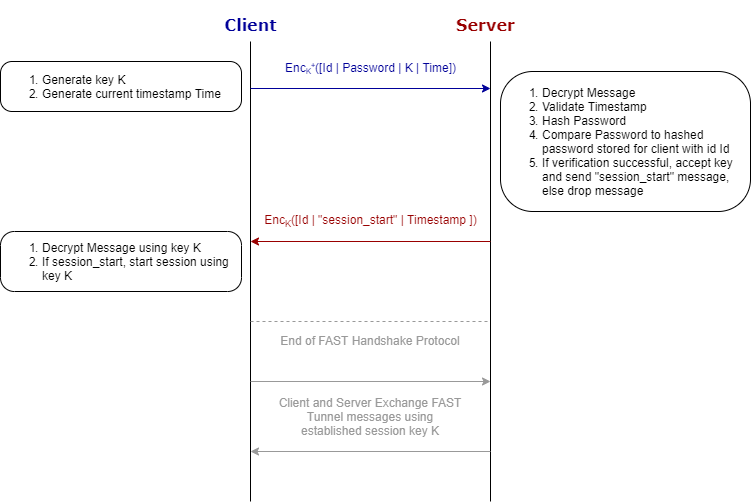
\includegraphics[width=\textwidth]{Handshake_MSC}
    \caption{Handshake protocol Message Sequence Diagram}
    \label{fig:handshake_msc}
\end{figure}

\subsubsection{Message Format and Message Processing Rules}

We describe the message formats and processing rules of this protocol in three phases

\paragraph{Phase 1: Initiation Message (Client)}

The Client initiates the protocol. The client sends the initiation message, which includes the client’s ID, the client’s Password, the client’s freshly generated key, and the client’s current timestamp, all encrypted with the server’s public key. The client does this in the following way:

\begin{enumerate}
    \item The client starts the message with its ID (32 bytes)
    \begin{itemize}
        \item The ID is a unique 32 byte value that uniquely identifies the client to the server
        \item The ID of a client is not a secret value
    \end{itemize}
    \item The client appends to the message its Password (32 bytes)
    \begin{itemize}
        \item The password is a secret value that only the client knows, which allows the server to authenticate the client
        \item The password must be at least 8 characters long, and must contain at least 1 lowercase letter, 1 uppercase letter, and 1 special character.
        \item Passwords cannot be longer than 32 characters
        \item Passwords use ASCII encoding. Passwords are not allowed to have non-ASCII characters
        \item All passwords, even if they are shorter than 32 characters, are sent in 32 bytes. If the password is shorter than 32 characters, the password is padded to make it fit into 32 bytes
        \item Passwords are padded using PKCS\#7 padding
    \end{itemize}
    \item The client generates a new fresh key and appends it to the message (32 bytes)
    \begin{itemize}
        \item The key generated must be a pseudorandom stream of 256 bits that can be used as a symmetric key for AES in GCM mode.
        \item The key must be generated with an appropriate cryptographic pseudo-random number generator
    \end{itemize}
    \item The client appends its timestamp (32 bytes)
    \begin{itemize}
        \item The client uses a timestamp format that is pre-agreed upon with the server (this is outside the scope of this protocol), but must be 32 bytes
    \end{itemize}
    \item The client encrypts the message
    \begin{itemize}
        \item The entire message (all 128 bytes) is preformatted for RSA encryption using PKCS\#1 v2 (OAEP)
        \item The client encrypts the preformatted message with the public key of the server, using RSA encryption 
    \end{itemize}
    \item The client sends the encrypted message to the server

\end{enumerate}

\paragraph{Phase 2: Verification, Session Creation, and Acknowledgement (Server)}

In this stage, the server decrypts the received message from the client. It verifies the timestamp and the password. If the client is authenticated, the server creates a new session with the client using the provided key, and sends an acknowledgement message to the client, encrypted with the new session key. Otherwise, the server drops the message and doesn’t send anything to the server. In detail, the server does the following:

\begin{enumerate}
    \item The server decrypts the message
    \begin{itemize}
        \item The server decrypts the message received from the client, using its private key
    \end{itemize}
    \item The server validates the timestamp
    \begin{itemize}
        \item The server checks that the timestamp is recent enough. Precisely, the server checks that the timestamp was from less than 1 minute ago. If the timestamp is fresh, verification resumes. Else, the message is dropped and the server goes back to waiting for another initiation message.
    \end{itemize}
    \item The server validates the password
    \begin{itemize}
        \item The server first removes the padding from the password
        \item The servers ensures that the password is valid
        \begin{itemize}
            \item  Shorter than 32 bytes and longer than 8 bytes
            \item Contains at least 1 character, 1 lowercase letter, and 1 uppercase letter
            \item Contains no non-ASCII characters
        \end{itemize}
        \item If the password is valid, the password is hashed
        \item Passwords are hashed using SHA-224
        \item The server looks up the password hash stored corresponding to the user ID provided, to the password hash just computed
        \item The hashed password is compared to the stored hash
        \item If the hashes match, the password is verified, and the client is authenticated. 
    \end{itemize}
    \item If the validation or authentication fails, drop the message
    \begin{itemize}
        \item If, at any stage in the previously mentioned steps of verification, validation, and authentication, that stage fails, the message is dropped, no message is sent to the client, and the server goes back to waiting for initiation messages.
    \end{itemize}
    
    \item If the verification and authentication succeeds, start the new session
    \begin{itemize}
        \item If all the previously mentioned steps succeed, the server accepts the new session with that client
        \item The server stores the new key K provided by the client in the current session field corresponding to the client ID
    \end{itemize}
    \item If the session is accepted, send an acknowledgement message	
    \begin{itemize}
        \item If the session is accepted, the following message is constructed:
        \item The ID of the client (provided by the client earlier) (32 bytes)
        \item The special message “session\_start” in ASCII (13 bytes)
        \item The current server’s timestamp (32 bytes)
        \item The full message (77 bytes) is encrypted
        \begin{itemize}
            \item Message is encrypted using symmetric key encryption with AES in GCM mode, using the newly established session key K as the symmetric key
            \item The Nonce used for this message is 1, signifying the first message sent using this session key
            \item The MAC length is 16 bytes
            \item There is no header associated data used. Instead, the entire message is encrypted
        \end{itemize}
        \item The generated ciphertext and tag are sent to the client
    \end{itemize}

\end{enumerate}

\paragraph{Phase 3: Session Start (Client)}

Once the client receives the “session\_start” message, it also accepts the new session, and stores the generated session key K in its state. It then starts communicating with the server using symmetric encryption with the key K.

\noindent When the client receives the message:

\begin{enumerate}
    \item Client decrypts and verifies the message
    \begin{itemize}
        \item If decryption and verification is unsuccessful, the message is dropped, and a new initiation message is sent with a new key, then client moves back to waiting for the acknowledgement message.
    \end{itemize}
    \item Client verifies message content
    \begin{itemize}
        \item The client verifies that the Id sent is its own ID, that the message is “session\_start”, and that the timestamp is within 1 minute ago.
        \item If this fails, the message is dropped, and we move back to waiting for the acknowledgement message.
    \end{itemize}
    \item Client accepts new session
    \begin{itemize}
        \item If all of the above is successful, the client accepts the new session, and starts sending commands to the server using the FAST Tunnel protocol, using the established symmetric key K.
    \end{itemize}
\end{enumerate}

If 5 minutes have passed since sending the initiation message, and the client has not received the session\_start message yet, the client drops the current session, and attempts to initiate a new session using a new freshly generated key.


This is the end of the FAST Handshake protocol, having established the session and the symmetric session keys. All further communication between the client and server uses the FAST Tunnel protocol.

\subsubsection{Cryptographic Primitives Used}

\paragraph{Asymmetric Key Encryption}

Used in sending the initiation message from client to server. Uses RSA public key encryption, with messages preformatted using PKCS\#1 v2 (OAEP). Public Key-Private Key pairs for the server are established beforehand and the public key communicated to the clients using a secure out-of-band channel, that is outside the scope of this protocol.

\paragraph{Padding}

Used to pad the password to be 32 bytes long. PKCS\#7 padding is used

\paragraph{Hashing}

Used to hash passwords. SHA-224 is used

\paragraph{Symmetric key encryption}

Used to send the session\_start message. AES in GCM mode is used, with 256-bit key, and the number 1 as the nonce (only 1 message is sent with this encryption). The MAC Length used is 16 bytes. No header data is used as associated data, since the entire message is encrypted.

\subsubsection{Protocol State Machine}

The following diagram summarizes the state machine and possible state changes for the server:

\begin{figure}[h]
    \centering
    \includegraphics[width=\textwidth]{Handshake_State_Diagram _Server}
    \caption{Handshake protocol server state diagram}
    \label{fig:handshake_state_server}
\end{figure}

\noindent Meanwhile, the following state machine diagram illustrates the states and state changes in the client

\begin{figure}[h]
    \centering
    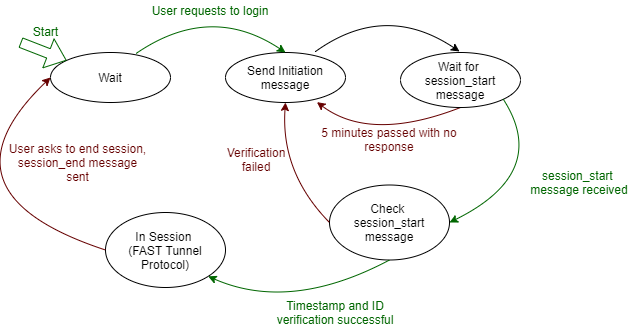
\includegraphics[width=\textwidth]{Handshake_State_Diagram_Client}
    \caption{Handshake protocol client state diagram}
    \label{fig:handshake_state_client}
\end{figure}

\subsection{FAST Tunnel Protocol}

\subsubsection{Overview}

The second protocol that we describe in this specification is the FAST Tunnel protocol. The FAST Tunnel protocol provides a secure channel that allows communication of commands between the client and the server. The FAST Tunnel protocol takes control as soon as the server switches to the “in session” state, as described earlier, and for the client as soon as it receives and validates the session\_start message. The FAST Tunnel is also responsible for the session\_end message, as illustrated in the state diagram above.

\subsubsection{Assumptions}

This protocol is initiated only after a successful handshake of the FAST Handshake protocol, having established a shared fresh session key. This protocol assume a shared session key is already established. Furthermore, The server is trustworthy. Lastly, both the client and the server, upon the start of the session, maintain a sequence number. It starts at zero when the session is first established.

\subsubsection{Message Sequence Diagram}

The following message sequence diagram describes at a high level the messages communicated using this protocol:
\newpage
\begin{figure}[H]
    \centering
    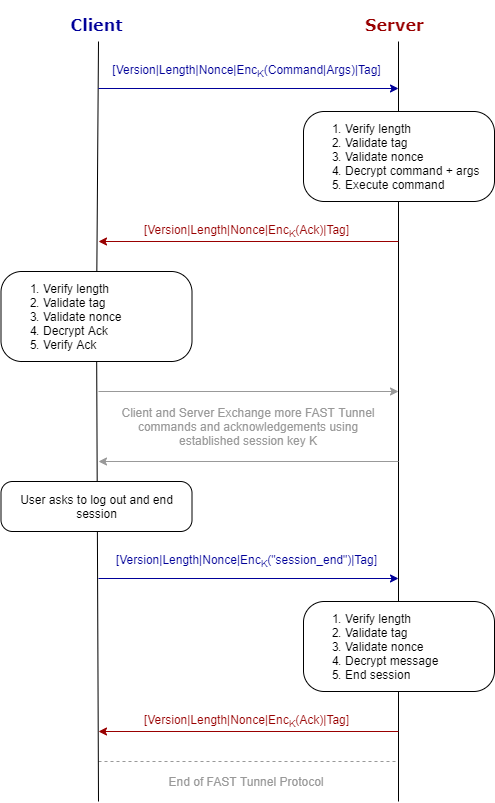
\includegraphics[scale=0.64]{Tunnel_MSC}
    \caption{Tunnel protocol message sequence diagram}
    \label{fig:tunnel_msc}
\end{figure}
\newpage

\subsubsection{Message Format}

All messages in this protocol take the following format (not to scale):

\begin{figure}[h]
    \centering
    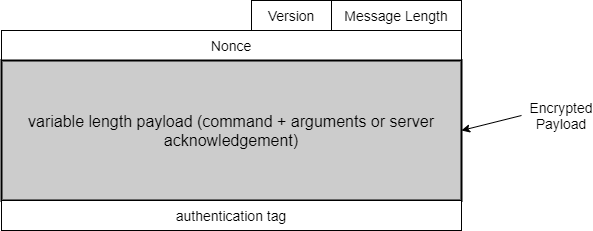
\includegraphics[width=\textwidth]{Message_Format}
    \caption{Tunnel protocol message format (not to scale)}
    \label{fig:tunnel_msc}
\end{figure}

\noindent where:

\paragraph{Version (2 bytes)}
Specifies the version number of the FAST Tunnel Protocol used. Each byte specifies a digit in the version number. For example, if the first byte is 1 and the second byte is 0, the version is interpreted as version 1.0

\paragraph{Message Length (4 bytes)}
Specifies the length of the full message. This length includes the whole message, including version number and message length bytes, as well as the authentication tag. This number is interpreted as integer using big endian encoding.

\paragraph{Nonce (16 bytes)}
These 16 bytes will be interpreted as an integer stored in big endian, and this number will be used as a nonce (N). N will serve two purposes: it acts as a message sequencing number to verify message order and prevent message replay, and will be used as the Nonce for encrypting the message and decrypting it on the receiving end, using AES encryption in GCM mode. N must be unique for each message in the session, and must be a strictly increasing counter. Messages will not be accepted if they have a lower Nonce than the most recently received Nonce.

\paragraph{Message Payload (variable length)}

This payload has two options. If the client is sending the message, it will be a command payload. If the server is sending the message, it will be an acknowledgment payload (with potential output). The exact format of the payload is described later. Regardless of how the payload is constructed, in both cases, the entire payload is encrypted using the session key K with AES encryption in GCM mode and 16 byte MAC.

\paragraph{Authentication tag (16 bytes)}

The 16 byte authentication tag returned from the AES encryption in GCM mode. Used to verify the authenticity and integrity of the message. The authenticated encryption scheme uses the header date (version, message length, and nonce) as the associated data, and the payload as the plaintext data to be encrypted.

\paragraph{Payload formatting}

\noindent The command payload is constructed as follows:

\begin{enumerate}
    \item Argument number (1 bytes)
    \begin{itemize}
        \item Specifies how many arguments the command has. The command itself counts as an argument. Therefore, the minimum number here is 1
    \end{itemize}
    \item Command (3 bytes)
    \begin{itemize}
        \item Specifies which command the client wishes to execute. Commands are three characters encoded in ASCII, and must be from the following
        \begin{itemize}
            \item MKD – creating a folder on the server
            \item RMD – removing a folder from the server
            \item GWD – asking for the name of the current folder (working directory) on the server
            \item CWD – changing the current folder on the server
            \item LST – listing the content of a folder on the server
            \item UPL – uploading a file to the server
            \item DNL – downloading a file from the server
            \item RMF – removing a file from a folder on the server
            \item END - a special command to end the current session. All sessions must end with this command
        \end{itemize}
    \end{itemize}
    \item Arguments (variable length)
    \begin{itemize}
        \item If more than one argument (the command) is provided, each extra argument must begin with 8 bytes specifying the size of the argument in bytes, followed by the argument itself. The argument size is interpreted as an integer encoded in big endian. 
        \item The following section specifies how many arguments each command expects
    \end{itemize}
\end{enumerate}

The acknowledgement message is constructed in a similar way except:

\begin{enumerate}
    \item Argument number signifies how many outputs the server is sending to the client. All commands, even if they don’t expect an output, receive the special output “acknowledged” (encoded in ASCII). This special output may be prepended to further output if appropriate. Therefore, the argument number as well must be at least 1
    \item The command is replaced with the special acknowledgement message “acknowledged”, encoded in ASCII (12 bytes)
    \item Any further outputs given by the server must, as before, begin with 8 bytes specifying the size of the output
    \item The outputs that the server will send will depend on the commands executed, as described in the following section

\end{enumerate}

\paragraph{Command Arguments and Outputs}

\begin{enumerate}
    \item MKD
    \begin{itemize}
        \item Arguments
        \begin{itemize}
            \item 1 extra argument follows the command
            \item File name: max 120 bytes
            \item Must be ASCII-encoded and cannot contain non-ASCII characters
        \end{itemize}
        \item Outputs
        \begin{itemize}
           \item If successful, 1 extra output: “success” (in ASCII)
           \item If failure, 2 extra outputs: “failure” in ASCII \& Error message in ASCII
        \end{itemize}
    \end{itemize}
    \item RMD
    \begin{itemize}
        \item Arguments
        \begin{itemize}
            \item 1 extra argument: file name or path
        \end{itemize}
        \item Outputs
        \begin{itemize}
           \item If successful, 1 extra output: “success” (in ASCII)
           \item If failure, 2 extra outputs: “failure” in ASCII \& Error message in ASCII
        \end{itemize}
    \end{itemize}
    \item GWD 
    \begin{itemize}
        \item No extra arguments
        \item outputs
        \begin{itemize}
           \item 1 extra output: the name of the current working directory (in ASCII)
        \end{itemize}
    \end{itemize}
    \item CWD
    \begin{itemize}
        \item Arguments
        \begin{itemize}
            \item 1 extra argument
            \item Directory path: max 120 bytes
            \item Must be ASCII-encoded and cannot contain non-ASCII characters
        \end{itemize}
        \item Outputs
        \begin{itemize}
           \item 1 extra output: the name of the new current working directory after executing the command (ASCII)
        \end{itemize}
    \end{itemize}
    \item LST 
    \begin{itemize}
        \item No extra arguments
        \item Outputs
        \begin{itemize}
           \item As many outputs as there are files/folders in the current directory. Each output will specify the name of the file/folder in ASCII
        \end{itemize}
    \end{itemize}
    \item UPL
    \begin{itemize}
        \item Arguments
        \begin{itemize}
            \item 2 extra argument
            \item File name: as before
            \item File: treated as binary blob, binary posted as-is to the current working directory under the given name
        \end{itemize}
        \item Outputs
        \begin{itemize}
           \item If successful, 1 extra output: “success” (in ASCII)
           \item If failure, 2 extra outputs: “failure” in ASCII \& Error message in ASCII
        \end{itemize}
    \end{itemize}
    \item DNL
    \begin{itemize}
        \item Arguments
        \begin{itemize}
            \item 1 extra argument: File Name or File Path:
        \end{itemize}
        \item Outputs
        \begin{itemize}
           \item 2 outputs: the file name in ASCII, and binary payload of the file (treated as a binary blob)
        \end{itemize}
    \end{itemize}
    \item RMF
    \begin{itemize}
        \item Arguments
        \begin{itemize}
            \item 1 extra argument: file name or path
        \end{itemize}
        \item Outputs
        \begin{itemize}
           \item If successful, 1 extra output: “success” (in ASCII)
           \item If failure, 2 extra outputs: “failure” in ASCII \& Error message in ASCII
        \end{itemize}
    \end{itemize}
    \item END
    \begin{itemize}
        \item No extra arguments
        \item No extra outputs
    \end{itemize}
\end{enumerate}


\subsubsection{Message Processing Rules}

\paragraph{Command Messages (Client to Server)}

Any interaction in this protocol is initiated by the client to execute a specific command. The Client initiates the protocol by sending a command message to the server, in the format described above.

\paragraph{Verification and Command Execution (Server)}

Once a command message is received by the server, the server authenticates the message using the tag provided. Then, the server validates the message sequence number (nonce). If it’s successful, the server decrypts the payload and executes the command. Once completed, the server sends an acknowledgement message and any output to the client, in the format described above. In detail, it works in the following way:

\begin{enumerate}
    \item The server validates the message sequence number
    \begin{itemize}
        \item In the same table that the server maps client IDs to password hashes and session keys, the server also stores a last received message sequence number (sqn), which is refreshed after each session, and starts at zero
        \item The server checks the nonce provided to the stored sqn
        \begin{itemize}
            \item If it’s higher, sqn is replaced with Nonce
            \item If it’s lower, the message is dropped and no further action is taken
        \end{itemize}
    \end{itemize}
    \item The server authenticates the message
    \begin{itemize}
        \item The server checks the authentication tag provided by the message. If authentication fails, the message is dropped and no further action is taken.
    \end{itemize}
    \item The server decrypts the payload
    \begin{itemize}
        \item The server uses the stored current session key, as well as the provided nonce, to decrypt the payload usinG AES in GCM mode.
    \end{itemize}
    \item Parse commands
    \begin{itemize}
        \item The server parses the payload following the command structure described above to extract the command requested and any additional arguments for the commands
    \end{itemize}
    \item Execute commands
    \begin{itemize}
        \item The server executes the command requested with the requested arguments using its existing file storage (this is outside the scope of this protocol)
        \item If the command is invalid, arguments are invalid, or command execution failed, the server sends an acknowledgement message with two extra outputs, specifying the appropriate error message, as specified above
        \item The server manages proper access rights based on the current session's user. This is outside the scope of this protocol.
        \item Any files uploaded by the users are handled as-is as binary blobs. The client may wish to encrypt or compress the files beforehand, but that is not handled by the server or by this protocol.
    \end{itemize}
    \item If execution successful, send appropriate acknowledgement message.

\end{enumerate}

\paragraph{Interpreting Acknowledgement Messages}

Upon reception of an acknowledgment message, the client verifies and decrypts the message, and extracts the output. The client also accepts acknowledgement numbers only if the received message nonce is strictly higher than the stored sqn.

To end the FAST Tunnel protocol, the client must send the special command “END” to the server, which prompts it to close the session. Upon reception of an acknowledgement message from an "END" command, the client logs out the user and deletes session keys.

\subsubsection{Cryptographic Primitives Used}

An authenticated encryption scheme is used to both authenticate and encrypt message payloads. AES in GCM mode is used, with 256-bit key, and the nonces sent in the header of the message. MAC Length used is 16 bytes. The header data (associated data used) is the version number, message length and nonce.

\subsubsection{Protocol State Machine}

The following diagram summarizes the state machine and possible state changes for the server:

\begin{figure}[H]
    \centering
    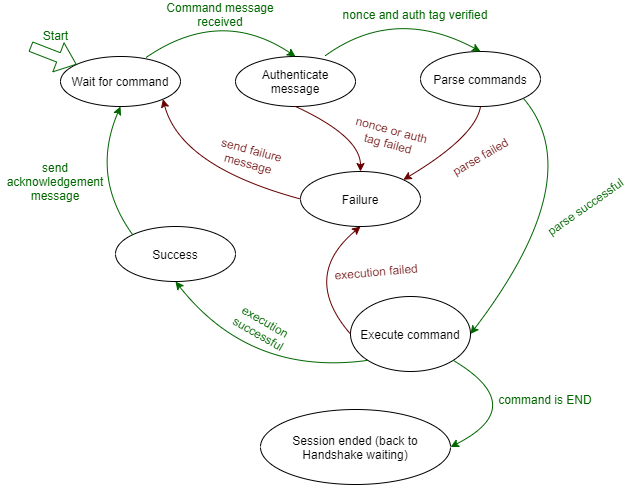
\includegraphics[width=\textwidth]{Tunnel_State_Diagram_Server}
    \caption{Tunnel protocol server state diagram}
    \label{fig:tunnel_msc}
\end{figure}

\noindent Meanwhile, the following state machine diagram illustrates the states and state changes in the client

\begin{figure}[H]
    \centering
    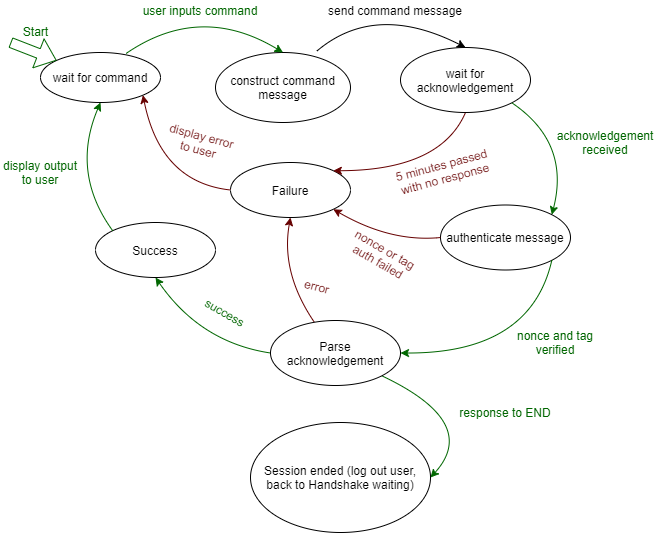
\includegraphics[width=\textwidth]{Tunnel_State_Diagram_Client}
    \caption{Tunnel protocol client state diagram}
    \label{fig:tunnel_msc}
\end{figure}

\section{Summary}

In the Handshake protocol, the confidentiality of the password is provided by the public key cryptography. Because the key is made available in a secure out-of-band channel, we can be sure of its security. Authenticity is provided by the password. Furthermore, replay protection and key freshness is guaranteed by the timestamp, since messages are only accepted if the timestamp falls within a certain short window.

In the second step, the authenticity and integrity of the start\_session message sent from the server to the client is guaranteed by the public key cryptography, since the server is guaranteed to be the only party, other than the client, to have access to the symmetric key. This is because the key was encrypted with the server’s public key, and therefore only the server can decrypt it and use it to encrypt an acknowledgement message. Furthermore, replay protection is similarly provided with the timestamp.

Therefore, the Handshake protocol satisfies all its securiry requirements and is able to establish a session key that only the server and the client have access to, to be used for secure communication over the secure channel in the Tunnel protocol.

In the Tunnel protocol, confidentiality of the messages, as well authentication and integrity protection, are provided by the securely established session key, since we use an authenticated encryption scheme, which implements both encryption and message integrity protection.

Furthermore, replay protection of message and message sequencing is handled by the nonce scheme, which is strictly increasing for each message and acts as a message sequence number. Non-repudiation of message origin is provided for both parties by the session key, since only the client and server have access to that shared key.

Therefore, the FAST Handshake and Tunnel protocols satisfy all our security requirements.




\end{document}
